%
% Sección de BPS.
% Artículo.
% Proyecto Lovelace.
%

\subsection{BPS}

% Borrador de la sección de BPS (v1)

Algoritmo de cifrado que preserva el formato capaz de cifrar cadenas formadas
por cualquier conjunto de caracteres, cuyo nombre proviene de las siglas de sus
autores Eric Brier, Thomas Peyrin y Jacques Stern; y que en el estándar
\cite{nist_fpe}, el NIST nombra como FF3.

BPS se conforma de 2 partes: un cifrado interno $BC$ que se encarga de cifrar
bloques de longitud fija, usando a su ves un cifrado por bloques $F$; y un modo
de operación especial, encargado de extender la funcionalidad del cifrado $BC$
y permitir cifrar cadenas de un longitud de hasta $max_b . 2^{16}$ caracteres,
donde $max_b$ es la longitud máxima que puede tener una cadena para cifrarse
con $BC$.

El cifrado interno utiliza una red Feistel y se define como $BC_{F,s,b,w}
(X,K,T)$ teniendo el proceso de cifrado descrito en la figura \ref{proceso_bc}.

\begin{figure}
  \begin{center}
    \begin{tabular}{|l|}
      \hline
      \begin{minipage}{0.5\textwidth}
        \begin{tabbing}
          \ \ \ \ \ \=\ \ \ \ \=\ \ \ \ \=\ \ \ \ \=\ \ \ \ \=\ \ \ \ \=\ \ \
          \ \kill \\
          \ \ \ \ {\bf Algoritmo} Cifrado $BC_{F,s,b,w}$($X$,$K$,$T$)\\
          \>  1. \> $T_R\: \gets\: T\: \mod\: 2^{32}$ y 
                    $T_L\: \gets\: (T\: -\: T_R) / 2^{32}$ \\
          \>  2. \> $l = r \gets b/2$ \\
          \>  3. \> $L_0\: \gets\: \sum_{j=0}^{l-1}\: X[j] \cdot s^j$ \\
          \>  4. \> $R_0\: \gets\: \sum_{j=0}^{r-1}\: X[j+l] \cdot s^j$ \\
          \>  5. \> {\bf para} $i=0$ {\bf hasta} $i=w-1$ \\
          \>  6. \> \> {\bf si} $i$ es par \\
          \>  7. \> \> \> $L_{i+1}\: \gets\: L_i\: \boxplus\: F_K((T_R \oplus i)
                          \cdot 2^{f-32}\: +\: R_i)\quad (mod\ s^l)$ \ \ \ \ \\
          \>  8. \> \> \> $R_{i+1}\: \gets\: R_i$ \\
          \>  9. \> \> {\bf si} $i$ es impar \\
          \> 10. \> \> \> $R_{i+1}\: \gets\: R_i\: \boxplus\: F_K((T_L \oplus i) 
                          \cdot 2^{f-32}\: +\: L_i)\quad (mod\ s^r)$ \ \ \ \ \\
          \> 11. \> \> \> $L_{i+1}\: \gets\: L_i$ \\
          \> 12. \> {\bf para} $i=0$ {\bf hasta} $i=l-1$ \\
          \> 13. \> \> $Y_L[i] \gets L_w\ mod\ s$ \\
          \> 14. \> \> $L_w \gets (L_w - Y_L[i])/s$ \\
          \> 15. \> {\bf para} $i=l$ {\bf hasta} $i=r-1$ \\
          \> 16. \> \> $Y_R[i] \gets R_w\ mod\ s$ \\
          \> 17. \> \> $R_w \gets (R_w - Y_R[i])/s$ \\
          \> 18. \> $Y \gets Y_L \parallel Y_R$ \\
        \end{tabbing}
        \end{minipage}\\
        \hline
      \end{tabular}
    \end{center}
    \caption{\label{proceso_bc} Cifrado interno BC.}
\end{figure}

Para cada bloque a cifrar, el cifrado $BC$ debe instanciarse con una longitud
de $max_b = 2 \cdot log_s(2^{f-32})$ caracteres, donde $f$ es número de bits
de salida del cifrado $F$, y $s$ es la cardinalidad del alfabeto usado por el
mensaje; y cuando la longitud total del mensaje a cifrar no sea múltiplo de
este valor, en el último bloque, $BC$ se tendrá que instanciar con una longitud
igual a la de ese bloque.

El modo de operación de BPS es un variación de CBC, con la diferencia de que
usa sumas modulares caracter por caracter en lugar de aplicar operaciones
\textit{xor}, además de que no emplea un vector de inicialización.
Otra característica es que utiliza un contador $u$ para aplicar una \textit{xor}
al \textit{tweak} $T$ que utiliza BPS.

El funcionamiento del modo de operación se describe en la figura \ref{modo_bps}.

\begin{figure}
  \begin{center}
    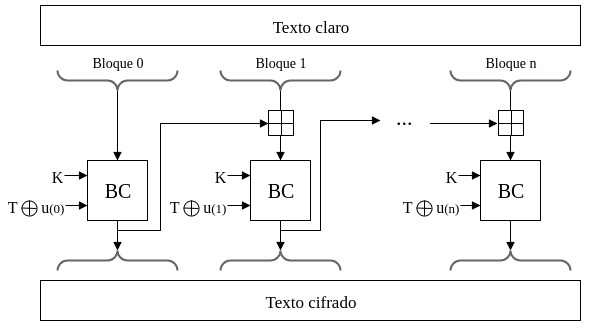
\includegraphics[width=0.85\linewidth]
    {../../../diagramas_comunes/bps/modo_de_operacion_bps}
    \caption{Modo de operación de BPS.}
    \label{modo_bps}
   \end{center}
\end{figure}
